\section*{Introduction}

This report explains the implementation details of CS523 Computer Vision
Assignment 2, which is about training a kNN classifier on the MNIST dataset,
reducing the dimensions with Principal Component Analysis(PCA) and using the
classifier on the Sudoku Dataset to recognize the digits. I will explain the
idea behind PCA for reducing the dimensions, the kNN classifier, processing
methods I have used to extract digits from the Sudoku Dataset and lastly comment
on my results.

To run the code, there needs to be an images directory where the .dat files and
.jpg files are located. Also
\href{https://pypi.org/project/python-mnist/} {python-mnist} needs to be
installed to load the MNIST dataset into numpy arrays.


\section*{Principal Component Analysis}

Principal Component Analysis(PCA) is an algorithm used for dimensionality
reduction. In the MNIST hand written digits dataset, each image comes as vectors
of dimension 784. However, we do not need all the dimensions contain classifying
an image.  The idea is, compressing a matrix with a lot of features into a
smaller matrix, with less features which preserves as much of the information in
the full matrix as possible.

In my PCA algorithm, to get the eigen vectors, I first calculated the mean
values of each column and centered the values I found by subtracting the mean
column value. Afterwards, I calculated the covariance matrix of the centered
matrix. Than, I calculated the eigen values and eigen vectors with and than
finally, sorted them with respect to their eigen value magnitudes.

To get the reduced versions of the images, I projected both train images and
test images on their first 25 principal components by a matrix multiplication.
To visualize the results, I used a function I found online to reconstruct the
first image of the MNIST dataset from its principal components and ended up with
the following image.

\begin{figure}[H] \centering
    \includegraphics[width=\textwidth]{images/before-after-pca.png}
    \caption*{PCA results} \setlength{\belowcaptionskip}{-40pt}
    \setlength{\abovecaptionskip}{-40pt}
\end{figure}

To observe the clustering, I projected the train images onto their first two
principal components and produced a scatter plot. 

\begin{figure}[H]
    \centering
    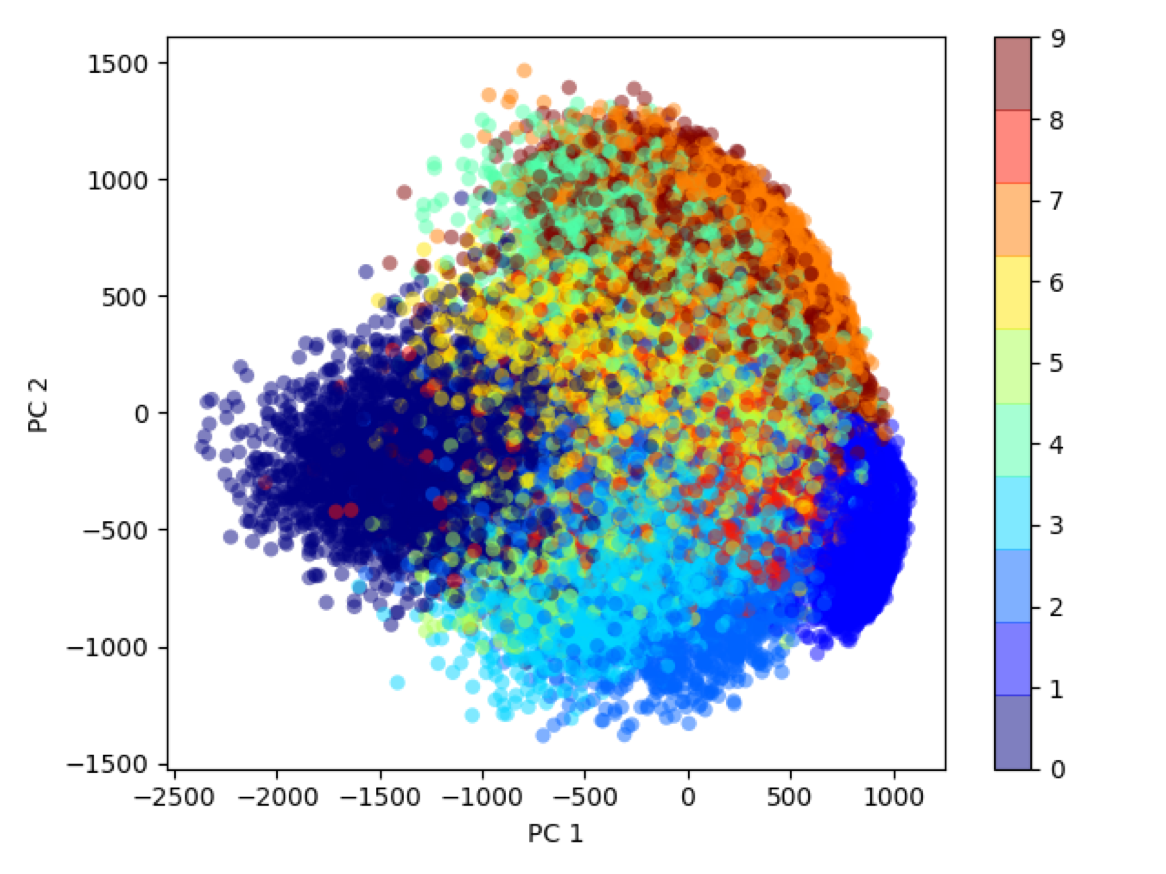
\includegraphics[width=\textwidth]{images/pca.png}
    \caption*{PCA results}
    \setlength{\belowcaptionskip}{-40pt}
    \setlength{\abovecaptionskip}{-40pt}
\end{figure}


\section*{k-Nearest Neighbor Algorithm}

k-Nearest Neighbors is a simple classification algorithm that stores all
available cases and classifies new cases based on a similarity measure.

After reducing the dimensions from 784 to 25, I computed the distances between
X\_test and X\_train to prepare my data for kNN classifier. To compute the
distances, I first used a nested for loop but ended up waiting 30 minutes for
computing the distances between train data and test data. To compute the
distances without any loops, I converted my nested for loops to a matrix
multiplication with two broadcast sums.

\begin{lstlisting}[language=Python, caption=Computing the distances without
loops]
    dists = np.reshape(np.sum(X**2, axis=1), [num_test,1]) + np.sum(X_train**2, axis=1) \
            - 2 * np.matmul(X, X_train.T)
    dists = np.sqrt(dists)

\end{lstlisting}

After computing the distances and obtaining a distance matrix, I looped over the
test data and used the distance matrix to find k nearest neighbors of the ith
testing point. Than I used the train labels to find the neighbors of the found
labels and than obtained the most common labels.

To find the best k value for the classification of the MNIST dataset, I looped
over k values from 0 to 15 and plotted the following graph to visualize my
findings. Lastly, I calculated the confusion matrix for 6 neighbors.

\begin{figure}[H]
    \centering
    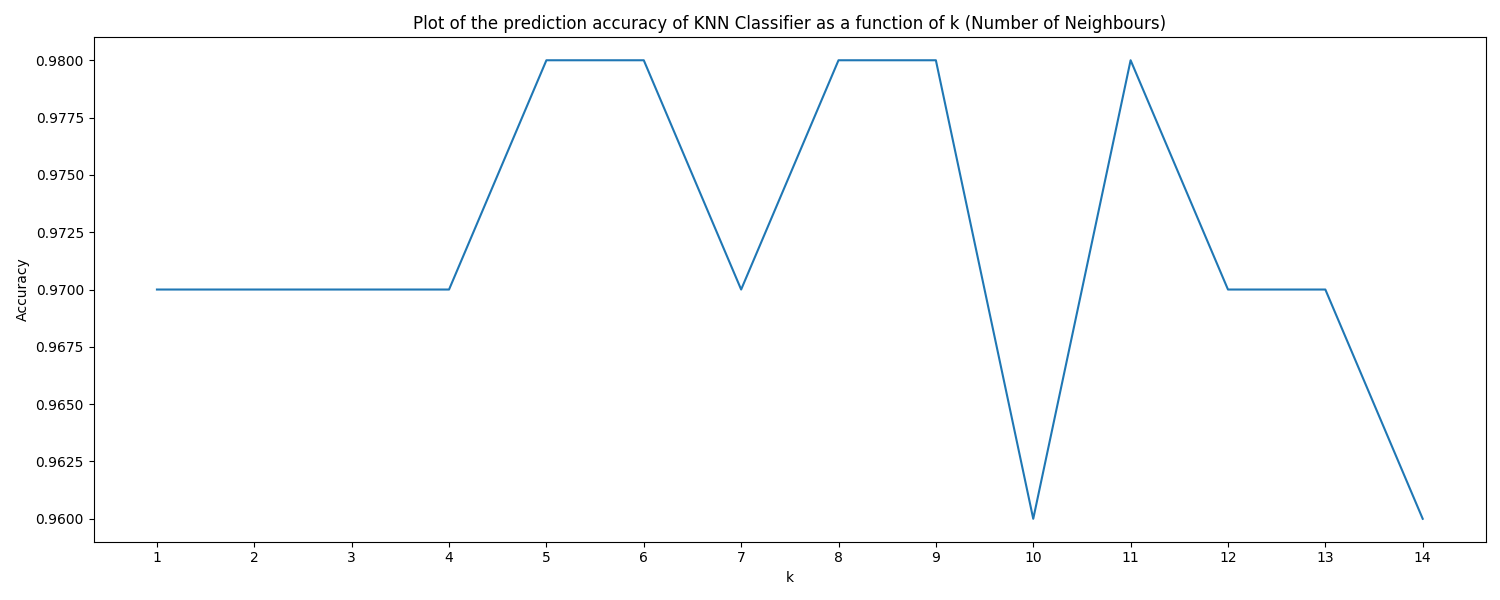
\includegraphics[width=\textwidth]{images/knn.png}
    \caption*{Prediction accuracy of kNN Classifier \\
    as a function of k (Number of Neighbours)}
    \setlength{\belowcaptionskip}{-20pt}
    \setlength{\abovecaptionskip}{-20pt}
\end{figure}


\begin{table}[H]
    \centering
    \begin{tabular}{llllllllllll}
        Predicted & 0 & 1     & 2     & 3     & 4    & 5    & 6    & 7     & 8    & 9    & All    \\
        Actual &      &       &       &       &      &      &      &       &      &      &        \\
        0      &  975 &     1 &     1 &     0 &    0 &    1 &    1 &     1 &    0 &    0 &    980 \\
        1      &    0 &  1131 &     1 &     0 &    0 &    0 &    3 &     0 &    0 &    0 &   1135 \\
        2      &    7 &     1 &  1003 &     0 &    1 &    0 &    3 &    11 &    6 &    0 &   1032 \\
        3      &    0 &     2 &     4 &   973 &    0 &   13 &    0 &     6 &   10 &    2 &   1010 \\
        4      &    0 &     0 &     0 &     0 &  960 &    0 &    4 &     2 &    0 &   16 &    982 \\
        5      &    3 &     2 &     1 &     9 &    1 &  868 &    5 &     1 &    1 &    1 &    892 \\
        6      &    4 &     4 &     0 &     0 &    3 &    0 &  947 &     0 &    0 &    0 &    958 \\
        7      &    1 &    20 &    10 &     0 &    2 &    0 &    0 &   985 &    0 &   10 &   1028 \\
        8      &    3 &     0 &     3 &    14 &    4 &    5 &    1 &     2 &  938 &    4 &    974 \\
        9      &    4 &     3 &     3 &    10 &   14 &    6 &    1 &     7 &    4 &  957 &   1009 \\
        All    &  997 &  1164 &  1026 &  1006 &  985 &  893 &  965 &  1015 &  959 &  990 &  10000 \\
    \end{tabular}
    \caption*{Confusion Matrix of kNN classifier with 6 neighbors\\
    Accuracy: 97.37\%}
\end{table}


\newpage

\section*{Sudoku Digit Extraction}

At the end of my assignment 1, I was able to find contours in a given sudoku
image. To use the kNN classifier on each digit on the Sudoku Dataset to get the
digits, I needed to do some processing. First I did a perspective transform to
obtain a bird eye view of the sudoku grid. 

Afterwards, I resized the image to 450 x 450 to iterate over it in 50 by 50 so
that I cover a cell with each iteration.

\begin{figure}[H]
    \centering
    \includegraphics[width=\textwidth]{images/wrapped.png}
    \caption*{Original,wrapped and Poorly Extracted Sudoku Grid}
    \setlength{\belowcaptionskip}{-20pt}
    \setlength{\abovecaptionskip}{-20pt}
\end{figure}

I iterated over image and extracted each 28 by 28 square. After some trial and
error, I decided to use the mean of each cell to determine if that cell is empty
or not. I created a 9 x 9 zero matrix to store the digit data, and marked the
non empty cells with -1. I projected each extracted cell to their first 25
principal components using the principal components I have computed at the
beginning. I repeated the steps that I have followed for computing the distances
and predicting the labels this time for the extracted pieces from the sudoku
grid.

Lastly I combined the prediction array and the grid array which resulted a final
9 x 9 array with my predictions and empty cells.

In the end U ended up with 38\% accuracy in the sudoku dataset.

\section*{Results}

I can say that the PCA for dimensionality reduction worked really well. In the
scatter plot, it is easy to see the clustering. The kNN algorithm also did a
great job in classifying the test images with an accuracy of 97.37\%.
Unfortunately sudoku predictions were not so well because of the existing grid
lines on extracted digits. With this project, I had a chance to understand the
power of the matrix multiplications since they helped me to reduce a process
which took 30 minutes to just a couple of minutes.

